\documentclass{standalone}

\usepackage{tikz}
\usepackage{graphicx}

\usetikzlibrary{automata, positioning, arrows}

\tikzset{
    ->,  % makes the edges directed
    >=stealth, % makes the arrow heads bold
    node distance=3cm, % specifies the minimum distance between two nodes. Change if necessary.
    every state/.style={thick, fill=gray!10}, % sets the properties for each ’state’ node
    initial text=$ $, % sets the text that appears on the start arrow
    }

\begin{document}
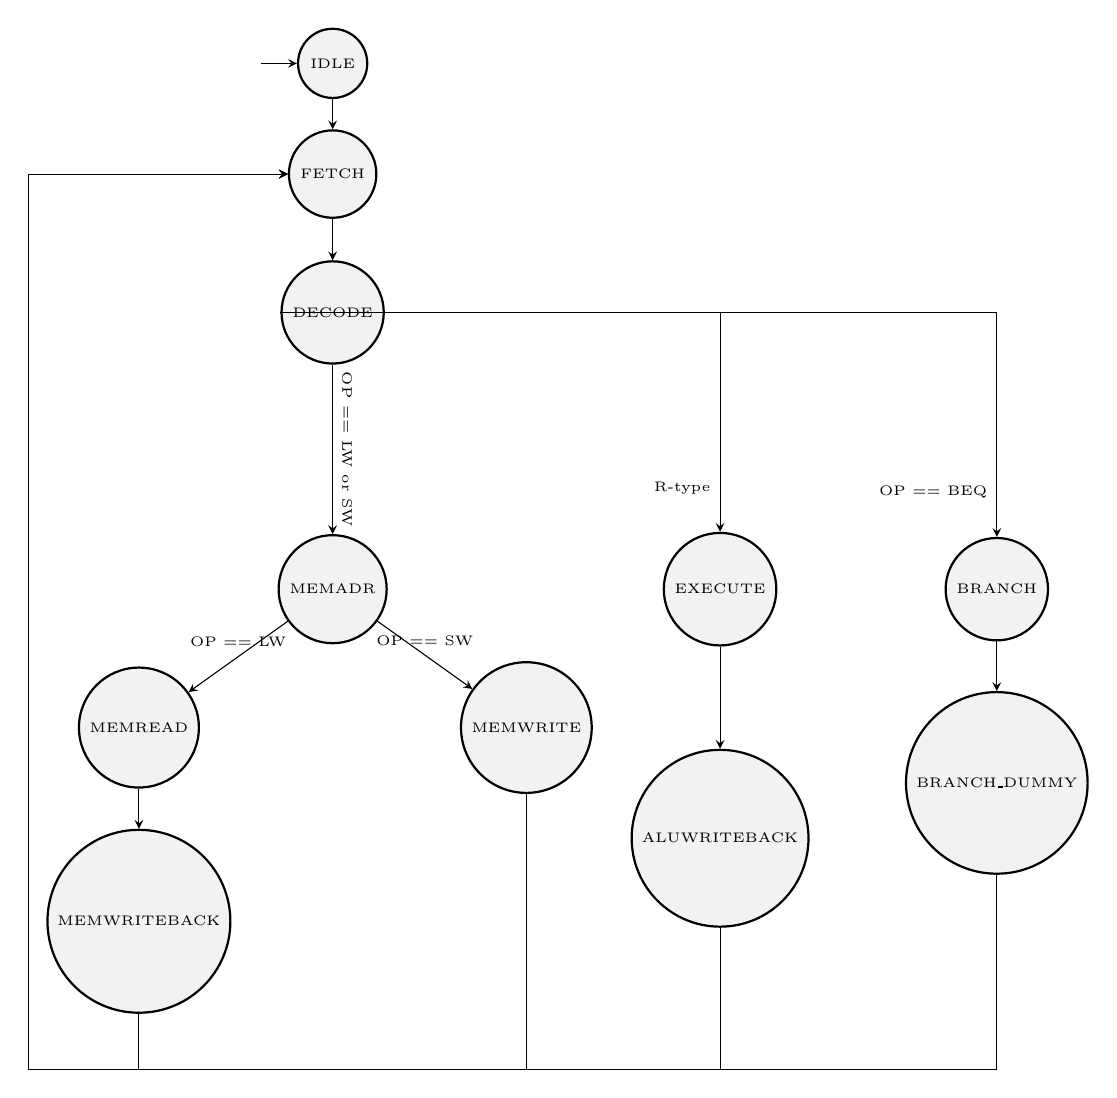
\begin{tikzpicture}
    \node[state, initial] at (0,0) (IDLE) {\tiny IDLE};
    \node[state] at ([xshift=0em,yshift=-4em]IDLE) (FETCH) {\tiny FETCH};
    \node[state] at ([xshift=0em,yshift=-5em]FETCH) (DECODE) {\tiny DECODE};
    \node[state] at ([xshift=0em,yshift=-10em]DECODE) (MEMADR) {\tiny MEMADR};

    \node[state] at ([xshift=-7em,yshift=-5em]MEMADR) (MEMREAD) {\tiny MEMREAD};
    \node[state] at ([xshift=7em,yshift=-5em]MEMADR) (MEMWRITE) {\tiny MEMWRITE};


    \node[state] at ([xshift=0em,yshift=-7em]MEMREAD) (MEMWRITEBACK) {\tiny MEMWRITEBACK};

    \draw (IDLE) edge[] (FETCH);
    \draw (FETCH) edge[] (DECODE);

    \draw (DECODE) edge[right] node{\rotatebox{-90}{\tiny OP == LW or SW}} (MEMADR);

    \draw (MEMADR) edge[above] node{\tiny OP == LW} (MEMREAD);
    \draw (MEMADR) edge[above] node{\tiny OP == SW} (MEMWRITE);
    \draw (MEMREAD) edge[]  (MEMWRITEBACK);

    \draw (MEMWRITEBACK.south) -- ([yshift=-2em]MEMWRITEBACK.south) -- ++ (-4em,0) |- (FETCH.west);

    \draw (MEMWRITE.south) |- ([yshift=-2em]MEMWRITEBACK.south) -- ++ (-4em,0) |- (FETCH.west);


    \node [state] at ([xshift=14em]MEMADR) (EXECUTE) {\tiny EXECUTE};
    \node[state] at ([yshift=-9em]EXECUTE) (ALUWRITEBACK) {\tiny ALUWRITEBACK};

    \draw (DECODE.east) -| (EXECUTE.north) node[pos=0.9,left] {\tiny R-type};
    \draw (EXECUTE.south) -- (ALUWRITEBACK.north);

    \draw (ALUWRITEBACK.south) |- ([yshift=-2em]MEMWRITEBACK.south) -- ++ (-4em,0) |- (FETCH.west);

    \node [state] at ([xshift=10em]EXECUTE) (BRANCH) {\tiny BRANCH};
    \node [state] at ([yshift=-7em]BRANCH) (BRANCHDUMMY) {\tiny BRANCH\_DUMMY};

    \draw (DECODE.west) -| (BRANCH.north)  node[pos=0.9,left] {\tiny OP == BEQ};

    \draw (BRANCH.south) -- (BRANCHDUMMY.north);
    \draw (BRANCHDUMMY.south) |- ([yshift=-2em]MEMWRITEBACK.south) -- ++ (-4em,0) |- (FETCH.west);

\end{tikzpicture}
\end{document}